\documentclass[12pt,letterpaper]{article}
\usepackage[utf8]{inputenc}

\usepackage{graphicx}
\setlength{\parskip}{0.4em}
\setlength{\parindent}{0em}

\begin{document}
\title{
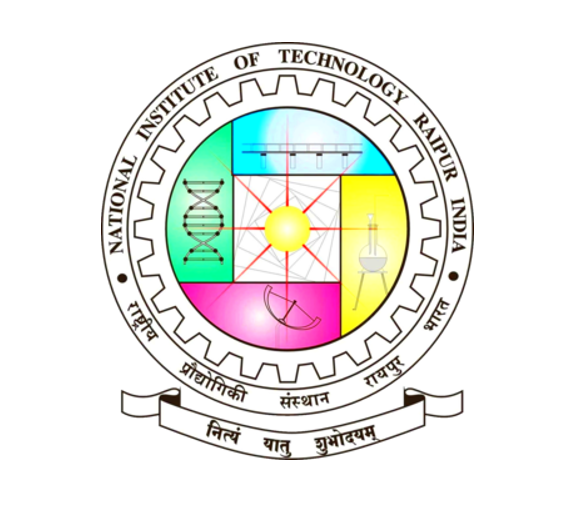
\includegraphics[width=0.3\textwidth]{National_Institute_of_Technology,_Raipur_Logo.png}
\\ 
Ancient Astronomy
}

\author{SHREEDUTT 19111056 BME 5TH SEMESTER}

\maketitle
\rule{\textwidth}{0.5pt}
\\
\subsubsection*{}
Let everyone be honest with the reality of today, \textbf{Artificial intelligence} is a \textbf{\textit{phrase}} that has taken several industries and professions by storm. Is it, however, still a \textbf{\textit{phrase}} that falls on deaf ears, or has it gained wide adoption and momentum?
\\
The term "Artificial Intelligence" has been associated with a variety of things over the years.
\\
\textbf{Healthcare}, E-Commerce, Mathematics, Medicine, and even \textbf{Immortality} are just a few instances. Clearly, the examples cover a large range of human imagination. However, there is one area that is relatively unexplored but equally exciting: \textbf{\textit{Artificial intelligence in Astronomy}}.
\\
\subsection* {AI in Astronomy} 
Understanding the Universe is critical in our quest to understand the origins of humans or life on Earth. And, in our quest to understand and find various answers, we become greedy, resulting in a flood of data that we don't know what to do with.
\\
\\
\textbf{\textit{According to Stanford researcher Andrew Ng, AI's capability is the ability to automate anything that a typical person can perform in less than one second of thought.}}
\\
\\
The next generation of AI astronomers aren't just interested in how this technology can sort data. They're looking into what could be an entirely new mode of scientific discovery, in which artificial intelligence maps out parts of the Universe we've never seen before.
\begin{center}
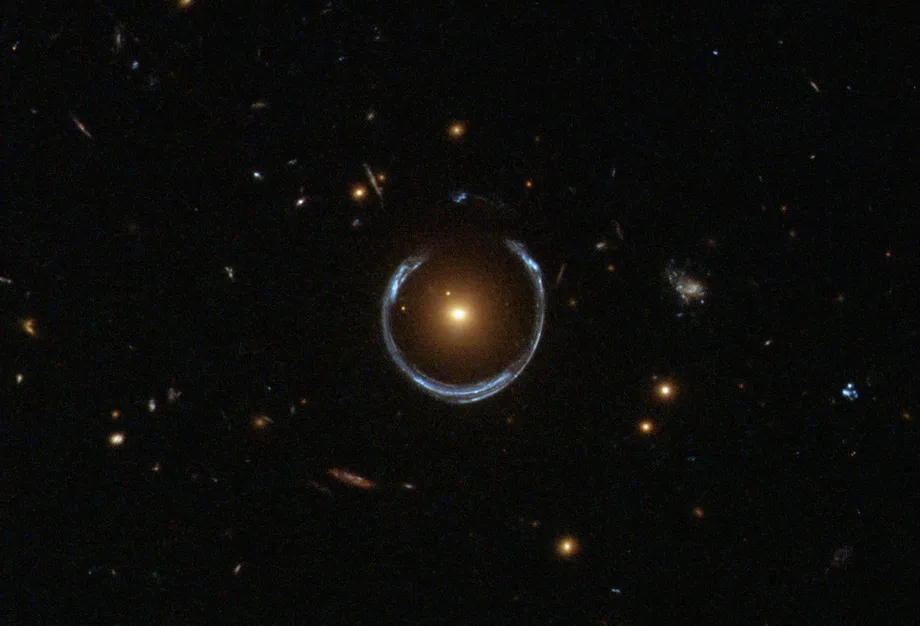
\includegraphics[width=0.6\textwidth]{gravitational_lens.png}
\\
\textit{A gravitational lens. The nearer red galaxy has bent the light of the more distant blue galaxy around it in a horseshoe shape.}
\end{center}
\\
Although Einstein's theory of general relativity predicted this phenomenon in the 1930s, the first example was discovered in 1979.space is huge, and looking at it takes a long time, especially without today's telescopes. As a result, the search for gravitational lenses has been haphazard so far.
\subsection* {Conclusion}
AI's application in Astrophysics is generating astronomical returns and redefining innovation in the world of Astro-Science, while also assisting in the discovery of some of the universe's greatest mysteries.
\\
Astronomers no longer need to burn the midnight oil straining their eyes to \textbf{detect, classify, and decode} spatial objects or hunt for new planets now that AI is being used to discover galaxies. We now have \textbf{\textit{AI-enabled super-telescopes}} that have their work cut out for them in the twenty-first century, and no one is complaining.
\end{document}
